%*************************************
% ภาคผนวก ง.
%*************************************
\appendixChapterTitle{ข}{สถาปัตยกรรมระบบและส่วนประกอบทางเทคนิค}
\section{สถาปัตยกรรมระบบและส่วนประกอบทางเทคนิค}
\hspace*{1.3em}
ระบบ Cloud-Based Platform ในฉบับปัจจุบันได้รับการออกแบบแบบ microservices และ multi-repository เพื่อให้แต่ละบริการสามารถพัฒนา ติดตั้ง และดูแลรักษาได้อย่างเป็นอิสระ ขณะที่ยังคงเชื่อมโยงกันผ่าน HTTP API, PostgreSQL, Redis และโครงสร้างพื้นฐานภายนอก

\vspace{0.5em}
\textbf{ภาพรวมสถาปัตยกรรมระบบ}
\vspace{0.5em}

\begin{figure}[htbp]
\centering
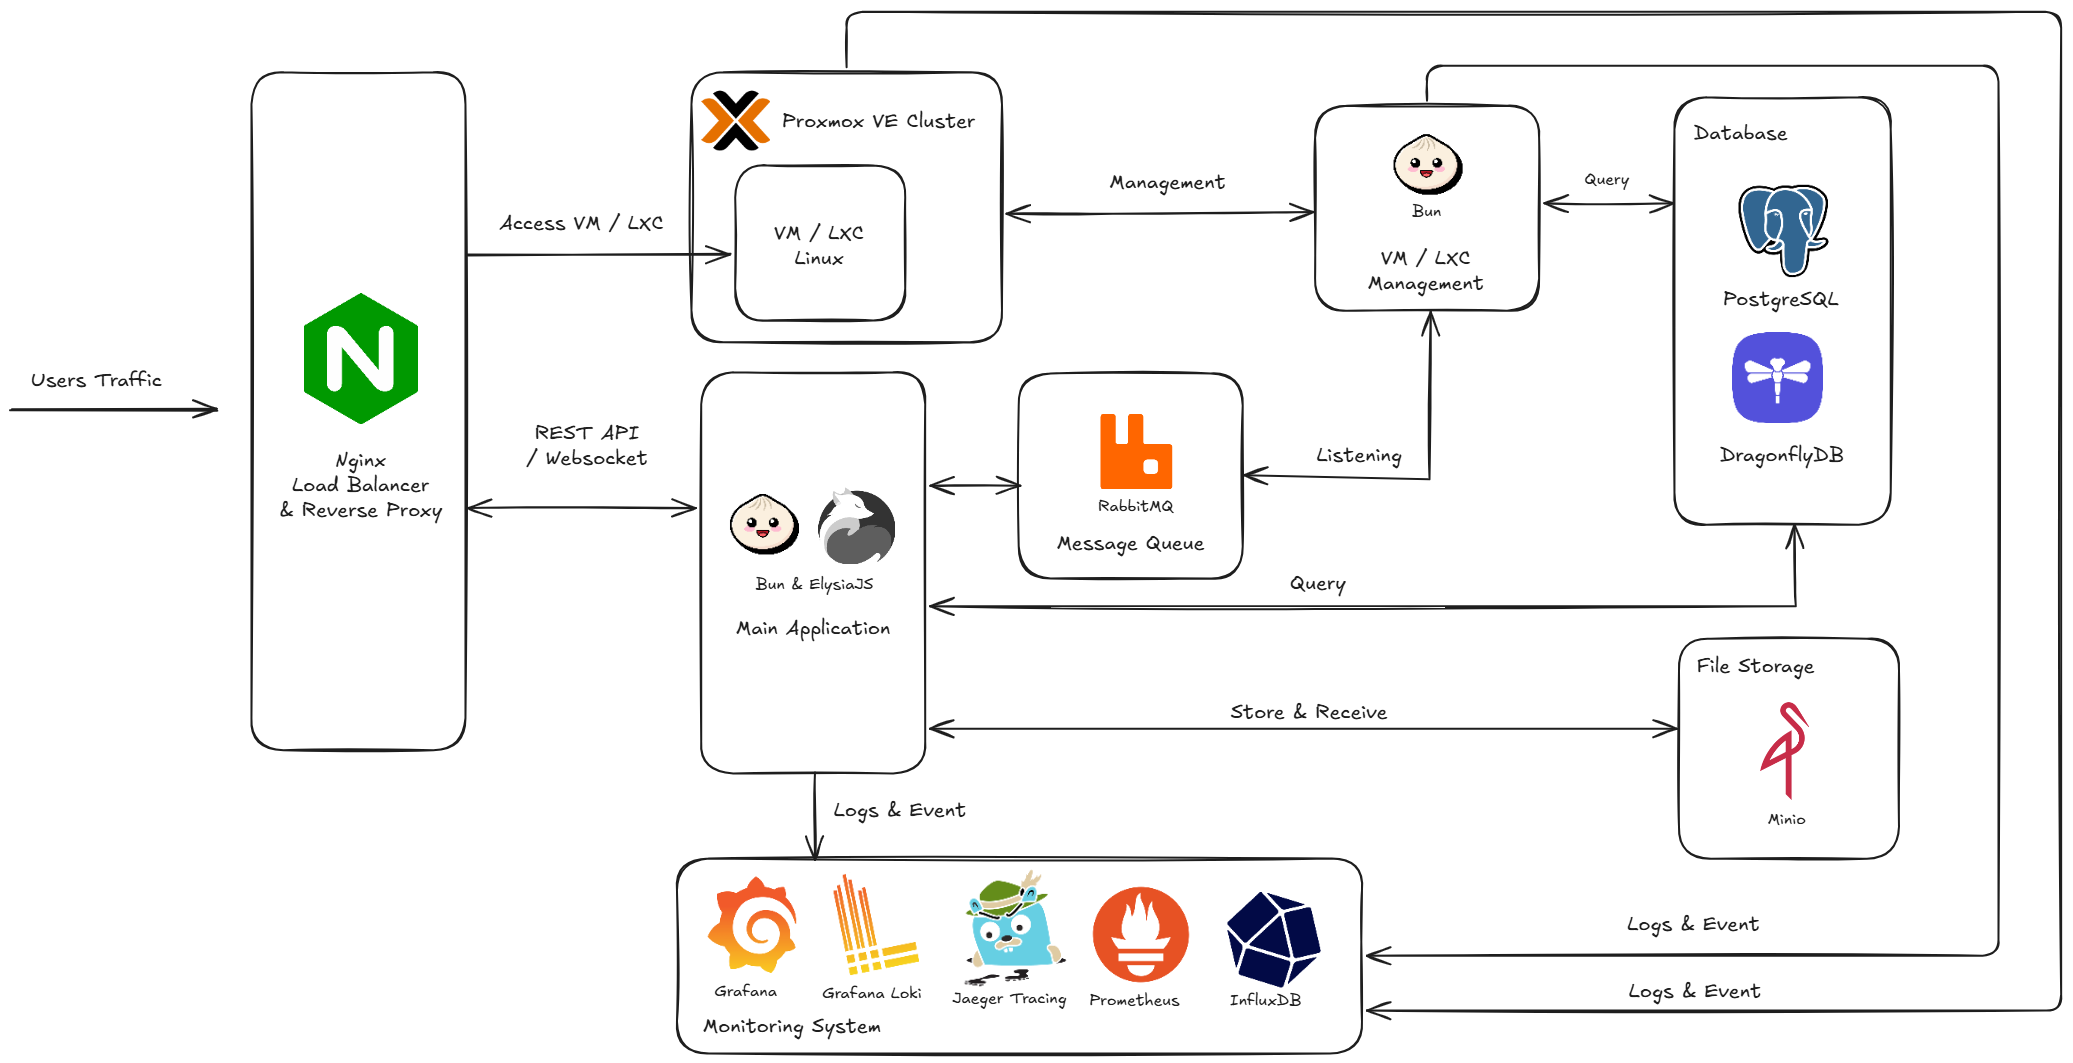
\includegraphics[width=0.9\textwidth]{./Image/web/system_architecture.png}
\caption{\fontSixTeen{สถาปัตยกรรมระบบ Cloud-Based Platform}}
\label{figD:SystemArchitecture}
\end{figure}

\section{บริการหลักและบทบาทในระบบ}
\hspace*{1.3em}
บริการหลักที่ใช้งานอยู่จริงใน code base ปัจจุบันมีดังนี้

\begin{mycustomenum2}
    \item \textbf{Midori} ทำหน้าที่เป็น frontend web application สำหรับนักศึกษา อาจารย์ และผู้ดูแลระบบ
    \item \textbf{Momoi} ทำหน้าที่เป็น API หลักของระบบ รับผิดชอบ business logic, OpenAPI, storage integration และ authentication endpoints
    \item \textbf{Yuzu} ทำหน้าที่เป็น background worker สำหรับจัดการ VM lifecycle บน Proxmox VE ผ่าน BullMQ
    \item \textbf{Satsuki} ทำหน้าที่เป็น automation service บนเครื่อง Nginx ภายนอก สำหรับสร้างไฟล์ reverse proxy configuration และ \textbf{authorized\_keys}
    \item \textbf{Yuuka} ทำหน้าที่เก็บ manifests, Docker Compose, observability configuration และเอกสารที่เกี่ยวข้องกับ deployment
\end{mycustomenum2}

\section{เทคโนโลยีที่ใช้ในการพัฒนา}
\hspace*{1.3em}
เทคโนโลยีที่ใช้งานจริงใน code base ปัจจุบันสามารถสรุปได้ดังนี้

\vspace{0.5em}
\textbf{Frontend Technologies}
\vspace{0.5em}

\begin{mycustomenum2}
    \item \textbf{Next.js 16} สำหรับพัฒนา Web Application แบบ React-based
    \item \textbf{React 19} สำหรับโครงสร้างส่วนติดต่อผู้ใช้
    \item \textbf{Tailwind CSS 4} สำหรับการจัดการรูปแบบหน้าจอ
    \item \textbf{TanStack React Query} สำหรับ data fetching และ state synchronization ฝั่ง client
    \item \textbf{better-auth client} สำหรับการเรียกใช้งาน authentication endpoints จากฝั่ง frontend
\end{mycustomenum2}

\vspace{0.5em}
\textbf{Backend และ Worker Technologies}
\vspace{0.5em}

\begin{mycustomenum2}
    \item \textbf{Bun} เป็น runtime หลักของ Momoi และ Yuzu
    \item \textbf{Elysia.js} เป็น web framework ของ Momoi
    \item \textbf{Prisma ORM} ใช้เข้าถึง PostgreSQL แบบ type-safe
    \item \textbf{PostgreSQL} เป็นฐานข้อมูลเชิงธุรกรรมหลักของระบบ
    \item \textbf{Redis} เป็น cache และ queue broker
    \item \textbf{BullMQ} เป็นระบบคิวงานระหว่าง Momoi และ Yuzu
    \item \textbf{better-auth} ใช้สำหรับ session และ OAuth flow ของระบบ
    \item \textbf{Zod} ใช้สำหรับ validation ของ environment variables และข้อมูลบางส่วนในระบบ
\end{mycustomenum2}

\vspace{0.5em}
\textbf{Virtualization และ Infrastructure}
\vspace{0.5em}

\begin{mycustomenum2}
    \item \textbf{Proxmox VE} เป็นแพลตฟอร์มหลักสำหรับจัดการ VM cluster
    \item \textbf{Kubernetes manifests} ในรีโพซิทอรี Yuuka ใช้สำหรับการติดตั้งบริการหลักในบางสภาพแวดล้อม
    \item \textbf{Docker Compose} ใช้สำหรับการเริ่มบริการประกอบในสภาพแวดล้อมพัฒนา
    \item \textbf{RustFS} ใช้เป็น S3-compatible object storage
    \item \textbf{Nginx} ทำหน้าที่เป็น reverse proxy หน้าด่านบนเครื่องภายนอก และรับการอัปเดต configuration จาก Satsuki
\end{mycustomenum2}

\section{ระบบคิวงานและการประมวลผลแบบ Asynchronous}
\hspace*{1.3em}
งานที่ใช้เวลานาน เช่น การสร้าง ลบ หรือเปลี่ยนสถานะ VM จะไม่ถูกประมวลผลภายใน request-response cycle ของ Momoi โดยตรง แต่จะถูกส่งเข้า Redis-backed BullMQ ก่อน จากนั้น Yuzu จะดึงงานไปประมวลผลแบบ asynchronous

\begin{mycustomenum2}
    \item \textbf{Provision Queue} สำหรับงานสร้าง VM ใหม่
    \item \textbf{Deprovision Queue} สำหรับงานลบหรือคืนทรัพยากรของ VM
    \item \textbf{Toggle Status Queue} สำหรับงาน Start, Stop และ Restart
\end{mycustomenum2}

\hspace*{1.3em}
ใน implementation ปัจจุบัน Yuzu รองรับการตั้งค่า concurrency แยกตามแต่ละคิวผ่าน environment variables และใช้ Redis-based distributed locks เพื่อกันงานที่ชน \textbf{instanceId} หรือ \textbf{VMID} เดียวกันไม่ให้ทำงานพร้อมกันโดยไม่จำเป็น

\section{Monitoring และ Observability}
\hspace*{1.3em}
ระบบมีการติดตามและตรวจสอบการทำงานอย่างครอบคลุมผ่านชุดเครื่องมือดังนี้

\begin{mycustomenum2}
    \item \textbf{Prometheus} สำหรับเก็บ metrics
    \item \textbf{Grafana} สำหรับสร้าง dashboards
    \item \textbf{Loki} สำหรับรวบรวม logs
    \item \textbf{Jaeger} สำหรับ distributed tracing
    \item \textbf{OpenTelemetry} เป็นมาตรฐานกลางสำหรับ telemetry data ของหลายบริการ
\end{mycustomenum2}

\section{ข้อดีของสถาปัตยกรรมที่เลือกใช้}
\hspace*{1.3em}
แนวทางสถาปัตยกรรมและเทคโนโลยีดังกล่าวมีข้อดีสำคัญดังนี้

\begin{mycustomenum2}
    \item แต่ละบริการสามารถพัฒนาและ deploy แยกกันได้ตามขอบเขตงาน
    \item Redis และ BullMQ ช่วยให้ระบบจัดการงานระยะยาวแบบ asynchronous ได้เหมาะสม
    \item การแยก Yuzu ออกจาก Momoi ช่วยลดภาระของ API หลักและเพิ่มความยืดหยุ่นในการ scaling
    \item Satsuki ช่วยทำให้ reverse proxy และ SSH access automation เชื่อมต่อกับข้อมูลในฐานข้อมูลได้โดยตรง
    \item OpenTelemetry, Prometheus และ Grafana ช่วยให้ติดตามปัญหาและวิเคราะห์ประสิทธิภาพของระบบได้ดีขึ้น
\end{mycustomenum2}
